\chapter{Objetivos}
Una vez que hemos enfocado el contexto en el que se va a desarrollar este trabajo, pasamos a definir el objetivo general y los subobjetivos que se pretender cubrir en este TFG.

El objetivo principal es desarrollar Classcity, una aplicación web desarrollada con tecnología de última  generación, cuya funcionalidad es facilitar el contacto entre alumnos y profesores para dar clases particulares. Classcity utiliza la geolocalización del alumno para proporcionarle los profesores más próximos a él, además de poder filtrar por diferentes parámetros como curso, asignatura y distancia.

\begin{figure}[H]
    \centering
    
\includegraphics[width=40mm]{memoria/LaTeX/img/introduccion/logo.jpg}
\end{figure}

Para la realización de esta aplicación hemos decidido dividir nuestro objetivo en sub-objetivos mas sencillos con la finalidad de que quitemos complejidad al proyecto. Estos sub-ojetivos son:
\begin{itemize}

    \item \textbf {Front-End}: La parte del cliente es quizás la más tediosa por su dificultad a la hora de desarrollar una interfaz lo suficientemente ligera y adaptable para diferentes tipos de dispositivo. Es por esto que la elección del framework en el cliente nos puede cambiar por completo la estructura de nuestra aplicación web, además de reducir mucho los tiempos de desarrollo.

    \item \textbf {Back-End}: El segundo sub-objetivo es plantearnos cual de los diferentes frameworks del backend se adaptan mejor a nuestras necesidades. La elección de este framework viene condicionado en gran medida por el framework seleccionado para el cliente.  
    
    \item \textbf {BBDD}: La base de datos por lo general pueden ser de dos tipos SQL y NoSQL, es por esto que debemos elegir cual de los dos tipos de bases de datos satisface mas con nuestras necesidades.
    
    \item \textbf {Despliegue en la nube}:Una vez que tengamos nuestra aplicación funcionando correctamente en local, es momento de desplegarlo en alguno de los cloud que nos ofrecen lo proveedores mas importantes como son: AWS, Azure o GoogleCloud 
    

\end{itemize}
\section{Metodología}
En la realización del proyecto se ha necesitado definir una metodología que permita planificar las tareas necesarias para llegar a nuestro objetivo. El modelo seleccionado para la ralización del TFG ha sido de tipo cascada, un proceso de desarrollo secuencial, en el que el desarrollo de software se concibe como un conjunto de etapas que se ejecutan una tras otra. Se le denomina así por las posiciones que ocupan las diferentes fases que componen el proyectom colocadas una encima de otra, y siguiendo un flujo de ejecuución de arriba hacia abajo, como una cascada.


\begin{figure}[H]
    \centering
    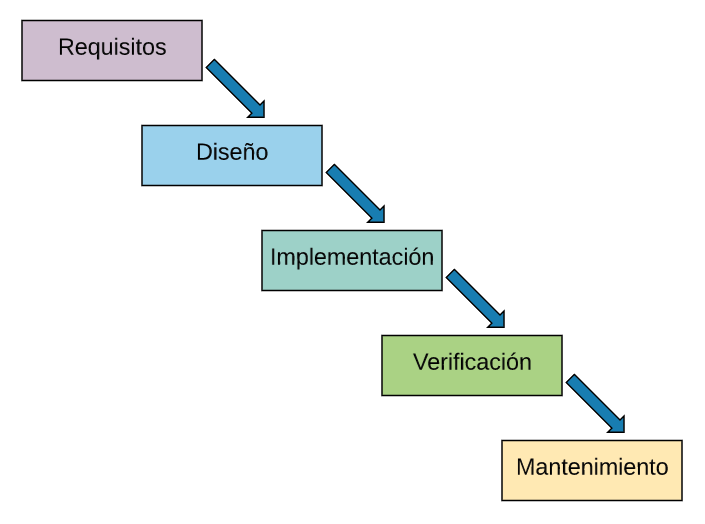
\includegraphics[width=100mm]{memoria/LaTeX/img/objetivos/cascada.png}
\end{figure}

Como parte de la metodología, durante el tiempo que ha durado el proyecto se acordaron reuniones semanales con el tutor de forma presenciales o por Vídeo-Conferencia en las que se revisaba los objetivos semanales y se definían los nuevos hitos.

\section{Plan de trabajo}

Para la realización de todo el proyecto he seguido una metodología de trabajo que ha consistido en cinco diferentes fases:

\begin{itemize}

\item \textbf {Primera fase}: Es una fase de iniciación cuyo objetivo principal es el de aprender todo lo que tenga que ver con el desarrollo web. En esta fase deberíamos de dejar conceptos básicos aclarados y empezar a manejar alguna herramienta de control de versiones como Git. Es muy recomendable en esta primera fase empezar a manejar los lenguajes de programación que quieras utilizar en el futuro.

\item \textbf {Segunda fase}: Una vez que tenemos cierta destreza con el desarrollo, empezamos a enfocar nuestra aplicación decidiendo que tecnologías son las que mejor nos van a venir para nuestro modelo de aplicación. Esta fase es vital para la continuación del proyecto, ya que la mala elección de una tecnología nos puede llevar mucho tiempo.

\item \textbf {Tercera fase}: Una vez que tenemos claro que tecnologías vamos a utilizar en nuestra aplicación, comenzamos con una sencilla aplicación que utilice todas las tecnologías que estarán implicadas en nuestra aplicación. Esto nos servirá para tener una sencilla estructura de lo que queremos montar.

\item \textbf {Cuarta fase}: Cuando tengamos claros los conceptos, manejemos los lenguajes de programación necesarios y tengamos montado una sencilla aplicación con las tecnologías que hemos seleccionado para nuestro proyecto, es momento de empezar a dar forma a nuestras ideas. Esta fase es quizás la más emocionante de todas ya que empiezas a dar cuerpo a lo aprendido hasta ahora. 

\item \textbf {Quinta fase}: Cuando tengamos nuestra aplicación completamente desarrollada y haciendo lo que nosotros queremos, es el momento de subirla a alguna plataforma de computación en la nube. Esta ultima fase es quizás la mas sencilla y mas gratificante del proceso ya que es el momento de que tu trabajo sea contemplado por el resto del mundo.

\end{itemize}



